\part{Introduction and Context}
\label{part:I}

\section{Introduction and Motivation}
\label{chap:intro}

\subsection{The Tension in Fundamental Physics: Time and Information}
The early 21st century finds fundamental physics in a state of productive tension. The partial unification achieved in the 1970s has bifurcated into two mutually incompatible frameworks: Quantum Mechanics (QM), describing the micro-world as probabilistic, unitary, and time-reversible; and General Relativity (GR), describing the macro-world as deterministic, geometrical, and background-independent. The interface between them---quantum gravity---remains elusive, primarily due to the "Problem of Time."
In GR, time is a dynamical coordinate found by solving the field equations (diffeomorphism invariance). In QM, time is a background parameter driving unitary evolution. The Wheeler-DeWitt equation $\hat{H}|\Psi\rangle = 0$, the naive quantization of GR, implies a "frozen formalism" where the physical state of a closed universe does not evolve.

Furthermore, the discovery of black hole thermodynamics and the holographic principle \cite{bekenstein1973black,hawking1975particle,susskind1995world} provides a sharp constraint/motivation: the information content of any finite spatial region is bounded by its surface area, not its volume. This suggests that the continuous manifolds of GR and the local fields of QFT may be redundant descriptions of a more fundamental, lower-dimensional organization of degrees of freedom.

This paper proposes a unified framework---\textbf{Omega Theory}---which addresses the time problem by accepting the static nature of the quantum universe (The Omega Axiom) and reinterpreting change as an intrinsic, operationally accessible structure on the state (projective geometry / information processing). This viewpoint is compatible with relational and thermal-time perspectives on ``evolution without external time'' \cite{PageWootters1983,ConnesRovelli1994}. We model the microscopic substrate as a discrete, finite-informational structure (a Quantum Cellular Automaton) together with a holographic encoding architecture for emergent effective spacetime descriptions.

\begin{figure}[h]
    \centering
    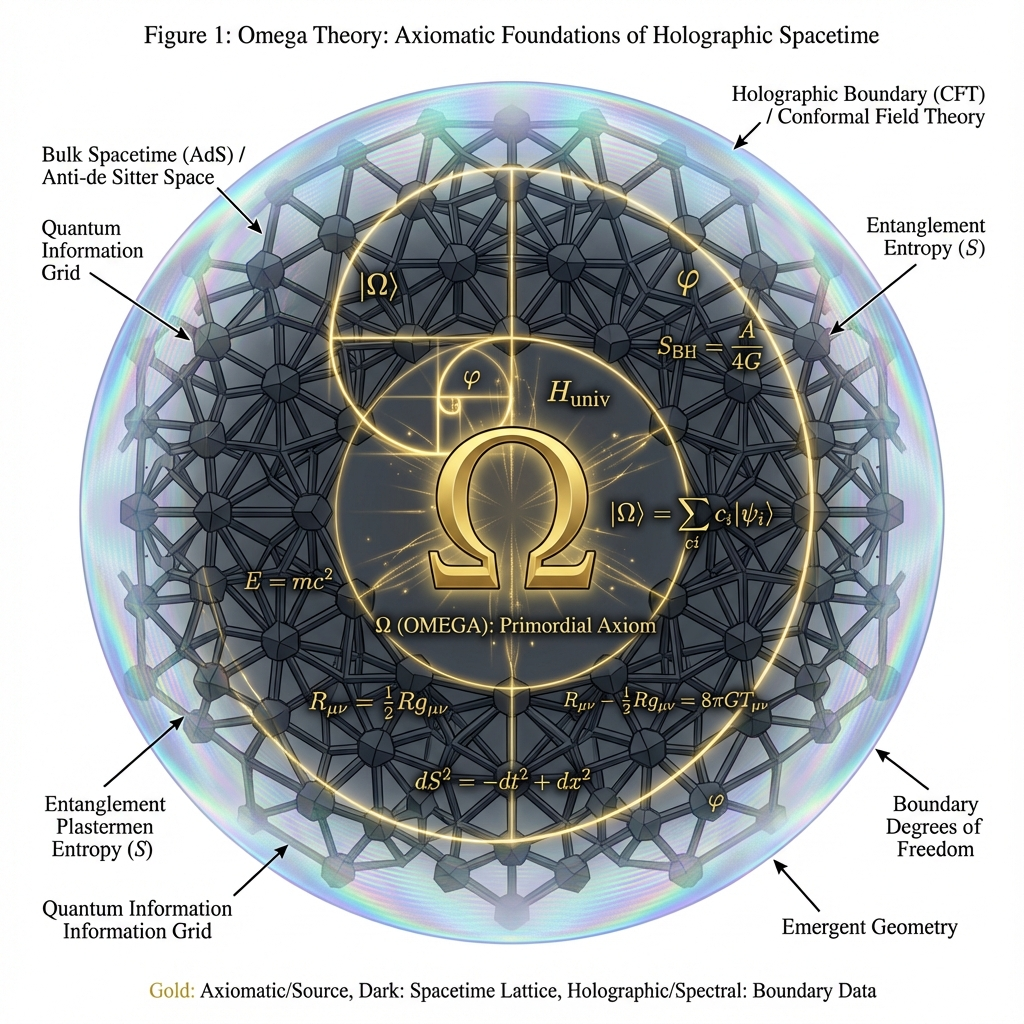
\includegraphics[width=0.8\textwidth]{images/omega_theory.png}
    \caption{Conceptual overview of Omega Theory: The static global vector $|\Omega\rangle$ yields an effective 4D spacetime description through holographic projection and quasicrystalline spectral/modular structure.}
    \label{fig:omega_concept}
\end{figure}

\subsection{Structure of the Argument}
Our argument proceeds in three layers, intended to separate rigorous foundations from specific models:
\begin{itemize}
    \item \textbf{Part I \& II (Foundations)}: We state the axioms around a global universe state $|\Omega\rangle$ and define intrinsic time via the geometry of projective Hilbert space (Fubini-Study metric). The finite-information/holographic input is treated as a working postulate that motivates an effectively discrete, local description.
    \item \textbf{Part III \& IV (Micro-Ontology)}: We propose a Quantum Cellular Automaton (QCA) on a quasicrystal network and analyze its Dirac continuum limit under explicit regularity assumptions. We then sketch how internal algebraic structure (octonions/$G_2$) could organize Standard Model-like quantum numbers, and we propose geometric ans\"atze for certain dimensionless constants.
    \item \textbf{Part V--VIII (Cosmology \& Interpretation)}: We introduce an information-geometric action principle (the Omega Action) and derive the associated field equations in a minimal setting. We outline cosmological/phenomenological consequences and discuss interpretational issues, including the role of observation in computationally incomplete dynamics.
\end{itemize}
For orientation, a compact dependency map of the main axioms, model assumptions, and derived templates is recorded in Appendix~\ref{sec:dependency_map}.

\section{Related Work and Positioning}
\label{chap:related_work}

Omega Theory does not exist in a vacuum. It synthesizes insights from several modern approaches but diverges in key ontological commitments.

\subsection{Relation to String Theory and AdS/CFT}
Like String Theory, we accept the Holographic Principle as central. However, unlike String Theory, which typically posits a background continuum (or an ensemble/landscape of vacua) and relies on string-scale excitations, Omega Theory is non-perturbative and background-independent from the start. Rather than invoking a landscape of distinct vacua, we postulate a single global state $\omega_\Omega$ (Axiom~O1); model-dependent ``vacuum data'' are encoded in the choice of that state and in the spectral/modular data of its restrictions to observer algebras.

\subsection{Relation to Loop Quantum Gravity (LQG)}
We share LQG's commitment to background independence and the discreteness of geometry (e.g.\ discrete spectra of kinematical area/volume operators) \cite{RovelliSmolin1995,AshtekarLewandowski1997Area}. However, deriving a fully controlled semiclassical limit together with a realistic low-energy matter sector remains challenging in current formulations; see, e.g., \cite{Perez2013SpinFoam,Thiemann2007}. Omega Theory sidesteps the direct quantization program by adopting a quantum-information substrate (a QCA) and treating both effective geometry and matter content as emergent in an appropriate coarse-grained limit.

\subsection{Relation to Causal Set Theory and Wolfram's Physics Project}
We share the vision that the universe is fundamentally a discrete graph or rewriting system (Causal Sets, Hypergraphs). However, most graph-based approaches struggle to recover quantum unitarity (the "Quantumness" problem). Omega Theory is strictly quantum-mechanical; the graph is treated as the tensor interaction structure of the Hilbert space, so microscopic unitarity is manifest in the regulated description.

\subsection{The Unique Contribution: Geometric Constants}
What sets Omega Theory apart is its attempt to relate dimensionless constants ($\alpha, \mu, \dots$) to geometric/topological data of the underlying informational construction, rather than treating them as arbitrary inputs. In this manuscript, these appear as explicit geometric ans\"atze; a full derivation from a unique microscopic measure and an explicit matching/RG closure remains an open task (Appendix~\ref{app:constants_proof}; Conjecture~\ref{conj:eft_matching}).

\subsection{Relation to Holographic Space-Time (HST) and Operator Algebras}
Omega Theory shares significant conceptual DNA with the \textbf{Holographic Space-Time (HST)} program of \textbf{Banks and Fischler} \cite{Banks2018}. Both approaches posit that spacetime is not fundamental but emerges from a finite quantum information structure, where the Hilbert space dimension determines the causal horizon area ($N \sim A/4G$). However, while HST constructs local causal diamonds dynamically, Omega Theory assumes a global static state $|\Omega\rangle$ from which causal diamonds are carved via tensor network disentanglers.

Furthermore, our identification of geometry with entanglement corresponds to the \textbf{Operator Algebra Quantum Error Correction (OAQEC)} framework \cite{Harlow2017, Pastawski2015}. The ``Golden MERA'' (Assumption~\ref{assump:M3}) is used here as a concrete tensor-network ansatz for the holographic encoding map postulated in Axiom~O4 \cite{Vidal2007MERA,Swingle2012MERA}, in the spirit of the HaPPY holographic pentagon code. The golden-spectrum update rule is an additional model assumption that supplies a specific intrinsic phase structure and a checkable dynamics/diagnostics layer for the ansatz, rather than a uniquely derived consequence of holography.

\section{Scope, Results, and Assumptions}
\label{chap:scope}

To facilitate verification, we state explicitly which elements are postulated, which are derived within the model, and which remain programmatic.

\subsection{Postulates (Axioms)}
\begin{itemize}
    \item \textbf{O1 (Omega Axiom)}: The universe is specified by a unique normalized global state $\omega_\Omega$ on a quasi-local operator algebra associated with a countable graph of finite-dimensional local degrees of freedom; there is no external time parameter \cite{BratteliRobinson1987OAQSM1}.
    \item \textbf{O2 (Finite Information)}: For any causally closed region with boundary area $A$, the effective dimension obeys $\dim \mathcal{H}_{\mathrm{region}} \le \exp(A/4l_P^2)$ \cite{bekenstein1973black,hawking1975particle,thooft1993dimensional,susskind1995world,Bousso2002}.
    \item \textbf{O3 (Causal Locality)}: There exists a discrete-time unitary update $\hat{U}$ with finite-range causal propagation: local observables evolve to observables supported only on bounded neighborhoods \cite{Watrous1995QCA,SchumacherWerner2004,Dariano2014}.
    \item \textbf{O4 (Holographic Mapping)}: There exists a holographic encoding map $\Phi$ from bulk to boundary which is an approximate isometry on the relevant code subspace and supports approximate OAQEC/entanglement-wedge reconstruction \cite{AlmheiriDongHarlow2015,Pastawski2015,Harlow2017}.
    \item \textbf{O5 (Scan--projection readout)}: Operational time and outcome statistics are obtained from finite-resolution scan and projection of intrinsic phase data (with standard consequences such as Sturmian readouts and canonical Ostrowski/Zeckendorf tick coordinates recorded as propositions in Part~II and Appendix) \cite{MorseHedlund1940,Lothaire2002,Zeckendorf1972,AlloucheShallit2003,Ma2025HPA}.
    \item \textbf{O6 (Unitary scan algebra)}: The scan is implemented by a nontrivial unitary $U_{\mathrm{scan}}$ with a conjugate unitary $V$ forming a Weyl pair, encoding intrinsic noncommutativity and uncertainty tradeoffs \cite{Weyl1916,Rieffel1981IrrationalRotations}.
\end{itemize}

\subsection{Model assumptions (concrete realization)}
\begin{itemize}
    \item \textbf{M1 (Icosahedral/quasicrystalline isotropy)}: The underlying graph is realized as an icosahedral quasicrystal ensuring statistical isotropy in the continuum limit (Assumption~\ref{assump:M1}).
    \item \textbf{M2 (Internal fiber and $G_2$ structure)}: Each site carries an $8$-dimensional internal sector organized by octonionic/$G_2$ structure (Assumption~\ref{assump:M2}).
    \item \textbf{M3 (Golden MERA / golden-spectrum update)}: A specific Golden MERA implementation of $\Phi$ and a golden-spectrum local update rule are adopted (Assumption~\ref{assump:M3}).
\end{itemize}

\subsection{Auxiliary assumptions}
\begin{itemize}
    \item \textbf{S1 (Readout-kernel symmetry)}: Microstate-counting normalizations assume a symmetric sharp-readout limit of the induced readout kernel (Assumption~\ref{assump:S1}).
    \item \textbf{C1 (Cosmological near-saturation)}: Cosmological scaling relations assume near-saturation of the holographic bound on horizon scales (Assumption~\ref{assump:C1}).
\end{itemize}

\subsection{Results derived in this manuscript (given the postulates)}
\begin{itemize}
    \item \textbf{Geometric time}: Intrinsic duration is identified with Fubini--Study distance in projective Hilbert space (Part II).
    \item \textbf{Omega Action variation}: A minimal information-geometric action yields modified Einstein equations with an ``information'' stress tensor, by direct variational calculus (Part V; Appendix \ref{app:action_proof}).
    \item \textbf{Dirac continuum limit (baseline and conditional extension)}: For the translation-invariant 1D coined walk, the long-wavelength limit yields Dirac evolution with a controlled lattice error (Part~III; Appendix~\ref{app:homogenization}). For quasicrystal/Fibonacci textures we provide explicit diagnostics on periodic approximants and quantify sensitivity to phason strain (Part~III; Appendix~\ref{app:fib_dqca}). The higher-dimensional homogenization target is isolated in Conjecture~\ref{conj:quasicrystal_dirac} and reduced to two quantitative control tasks in Appendix~\ref{app:homogenization}, Proposition~\ref{prop:quasicrystal_homogenization_reduction}.
\end{itemize}

\subsection{Programmatic components and open problems}
We isolate the remaining programmatic tasks into checkable reductions:
\begin{enumerate}
    \item \textbf{QFT locality vs.\ finite factorization (split-property target).}
    Continuum AQFT local algebras are typically type~III and do not admit an exact tensor factorization, while the regulated/QCA description is type~I on finite code subspaces. A controlled bridge requires an explicit effective-limit framework (Appendix~\ref{app:formal_proofs}).\par
    \textit{Minimal verification criteria.} Establish an approximate split-property statement at finite resolution (existence of intermediate type~I factors for nested regions) and identify the scaling regime in which the code-subspace description reproduces continuum correlators to a stated accuracy \cite{Haag1996,Buchholz1987}.

    \item \textbf{Fermion doubling and gauge structure (spectral/anomaly target).}
    The projection-filter mechanism is designed to gap would-be doublers while preserving a controlled low-energy Dirac sector (Appendix~\ref{app:doubling_filter}); the octonionic/$G_2$ organization supplies representation-theoretic constraints and anomaly conditions (Part~IV; Lemma~\ref{lemma:sm_anomaly_cancellation}).\par
    \textit{Minimal verification criteria.} Provide a higher-dimensional spectral analysis that quantifies doubler gaps and chiral content in the relevant quasicrystal/QCA setting (beyond the 1D testbed), and verify that the induced low-energy gauge sector satisfies the anomaly constraints and admits consistent Yukawa textures \cite{Nielsen1981,PeskinSchroeder1995}.

    \item \textbf{Geometric constants (matching and measure target).}
    The working geometric values for $\alpha^{-1}$ and $\mu$ are treated as matching data; closing this sector requires specifying a microscopic measure/coarse-graining scheme that produces definite boundary conditions at a scale $\mu_\ast$ and then propagating them by standard EFT/RG flow (Appendix~\ref{app:constants_proof}; Conjecture~\ref{conj:eft_matching}).\par
    \textit{Minimal verification criteria.} Specify the measure data that fixes the matching constants, quantify the induced threshold spectrum, and run the resulting EFT to laboratory scales within stated error budgets \cite{PeskinSchroeder1995}.

    \item \textbf{Observation and incompleteness (operational map target).}
    The observer/selection layer is intended as an operational map on a quasi-local algebra rather than as an additional dynamical postulate; its role is to formalize how computationally undecidable questions can arise for sufficiently expressive local dynamics (Part~VII; Appendix~\ref{app:formal_observation}).\par
    \textit{Minimal verification criteria.} Specify $\hat{\mathcal{O}}$ as a standard quantum operation (POVM/CPTP instrument) on the relevant effective algebra, exhibit a universal-computation embedding for the regulated dynamics, and show that the associated reachability/decision questions reduce to classical undecidable problems in the appropriate subspace \cite{NielsenChuang2000,Moore1990Unpredictability,Kari1994Reversibility,CubittPerezGarciaWolf2015SpectralGap}.
\end{enumerate}
